\documentclass[acmtog, nonacm, language=english, language=greek]{acmart}

\usepackage{alphabeta}
\usepackage[utf8]{inputenc} % Required for inputting international characters
\usepackage[T1]{fontenc} % Use 8-bit encoding


\usepackage{tikz}
\usepackage{dirtytalk}
\usepackage{smartdiagram}
\usetikzlibrary{shapes.geometric, arrows}
% \usetikzlibrary{timeline}



\tikzstyle{startstop} = [rectangle, rounded corners, minimum width=3cm, minimum height=1cm,text centered, draw=black, fill=red!30]
\tikzstyle{io} = [trapezium, trapezium left angle=70, trapezium right angle=110, minimum width=3cm, minimum height=1cm, text centered, draw=black, fill=blue!30]
\tikzstyle{process} = [rectangle, minimum width=3cm, minimum height=1cm, text centered, draw=black, fill=orange!30]
\tikzstyle{decision} = [diamond, minimum width=3cm, minimum height=1cm, text centered, draw=black, fill=green!30]
\tikzstyle{arrow} = [thick,->,>=stealth]


\newcommand{\en}[1]{\textlatin{#1}}
\newcommand{\src}[1]{\texttt{\en{#1}}}

%%
%% \BibTeX command to typeset BibTeX logo in the docs
\AtBeginDocument{%
  \providecommand\BibTeX{{%
    Bib\TeX}}}

%% Rights management information.  This information is sent to you
%% when you complete the rights form.  These commands have SAMPLE
%% values in them; it is your responsibility as an author to replace
%% the commands and values with those provided to you when you
%% complete the rights form.
\setcopyright{acmcopyright}
\copyrightyear{2022}
\acmYear{2022}
\acmDOI{}



%% If you are preparing content for an event
%% sponsored by ACM SIGGRAPH, you must use the "author year" style of
%% citations and references.
\bibliographystyle{ACM-Reference-Format}



%%
%% end of the preamble, start of the body of the document source.
\begin{document}

%%
%% The "title" command has an optional parameter,
%% allowing the author to define a "short title" to be used in page headers.
\title{Σχεδιασμός και Υλοποίηση Ιστοσελίδας Υποστήριξης Κοινότητας}

%%
%% The "author" command and its associated commands are used to define
%% the authors and their affiliations.
%% Of note is the shared affiliation of the first two authors, and the
%% "authornote" and "authornotemark" commands
%% used to denote shared contribution to the research.
\author{Ευάγγελοσ Λάμπρου}
\email{e.lamprou@upnet.gr}
\orcid{}
\affiliation{%
  \institution{Πανεπιστήμιο Πατρών}
  \streetaddress{}
  \city{}
  \state{}
  \country{}
  \postcode{}
}

\author{Απόστολος Παπαδημητρίου}
\affiliation{%
  \institution{Πανεπιστήμιο Πατρών}
  \streetaddress{}
  \city{}
  \country{}}
\email{a.papadimitriou@upnet.gr}

%% The abstract is a short summary of the work to be presented in the
%% article.
\begin{abstract}
    Στα πλαίσια αυτής της εργασίας γίνεται ο σχεδιασμός και η υλοποίηση μίας 
    ιστοσελίδας Υποστήριξης Κοινότητας. Γίνεται ανάλυση των απαραίτητων 
    λειτουργιών για την εφαρμογή και περιγράφεται το σύνολο των τεχνολογιών 
    που χρησιμοποιήθηκαν με εστίαση σε αξιοσημείωτα μέρη της υλοποίησης.
\end{abstract}

\maketitle

\section{Εισαγωγή}

\section{Εννοιολογικός Σχεδιασμός}

\subsection{Λειτουργικές Απαιτήσεις}

Έχοντας διαλέξει τον στόχο της εργασίας μας, συγκρίναμε άλλες εφαρμογές τύπου \en{Forum} και παρατηρήσαμε τις πιο χρήσιμες λειτουργίες.
Μαζί με τις λειτουργίες που θεωρήσαμε πιο χρήσιμες προσθέσαμε και τις λειτουργίες που χρειαζόμασταν προκειμένου η εφαρμογή μας να ανταποκρίνεται στις απαιτήσεις μας.

\subsubsection{Βασικές λειτουργίες}
\begin{itemize}
    \item Κεντρική Σελίδα
    \item Προφίλ Χρήστη
    \item Δημιουργία και σύνδεση νέου Χρήστη
    \item \en{Session} Χρήστη
    \item Σελίδα δραστηριοτήτων
    \item Εγγραφή και απεγγραφή σε δραστηριότητες
    \item Δημιουργία αναρτήσεων
    \item Σχολιασμός αναρτησεων
\end{itemize}

\subsubsection{Εξτρά λειτουργίες}
\begin{itemize}
    \item Δημιουργία φιλων
    \item Άντληση ενδιαφέρων στατιστικών
    \item Μοναδικές εικόνες προφίλ
    \item Απάντηση σε σχόλια
    \item Εμφανιση κειμενου σε \en{Markdown}
    \item Λειτουργίες διαχειριστων κοινοτητας (Εισαγωγή νέων δραστηριοτήτων, Διαγραφή σχολίων κτλπ.)
\end{itemize}

\subsection{Βάση Δεδομένων}
\subsection{Διάγραμμα Ροής Χρήστη}

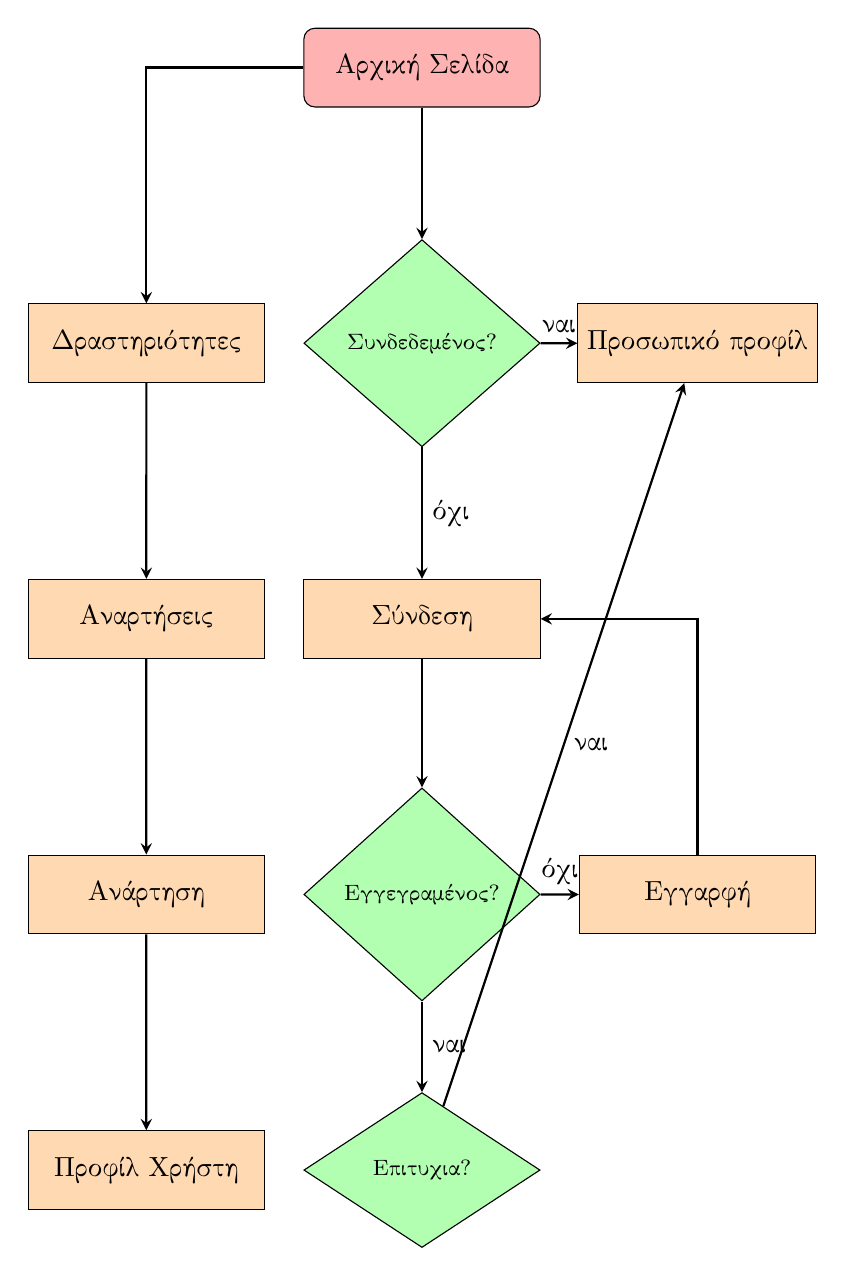
\begin{tikzpicture}[node distance=3.5cm, scale=0.6, every/.style={transform shape}]

    \node (start) [startstop] {Αρχική Σελίδα};

    \node (loggedin)        [decision, below of=start]         {\footnotesize Συνδεδεμένος?};
    \node (activitiespage)  [process, left of=loggedin]        {Δραστηριότητες};
    \node (postspage)       [process, below of=activitiespage] {Αναρτήσεις};
    \node (postpage)        [process, below of=postspage]      {Ανάρτηση};
    \node (profile)         [process, below of=postpage]       {Προφίλ Χρήστη};
    \node (loginpage)       [process, below of=loggedin]       {Σύνδεση};
    \node (registered)      [decision, below of=loginpage]     {\footnotesize Εγγεγραμένος?};
    \node (loginsucess)     [decision, below of=registered]    {\footnotesize Επιτυχια?};
    \node (registerpage)    [process, right of=registered]     {Εγγαρφή};
    \node (personalprofile) [process, right of=loggedin]       {Προσωπικό προφίλ};

    \draw [arrow] (start)          -- (loggedin);
    \draw [arrow] (start)          -| (activitiespage);
    \draw [arrow] (loggedin)       -- node[right] {όχι} (loginpage);
    \draw [arrow] (loggedin)       -- node[above] {ναι} (personalprofile);
    \draw [arrow] (loginpage)      -- (registered);
    \draw [arrow] (registered)     -- node[above] {όχι} (registerpage);
    \draw [arrow] (registered)     -- node[right] {ναι} (loginsucess);
    \draw [arrow] (loginsucess)    -- node[right] {ναι} (personalprofile);
    \draw [arrow] (registerpage)   |- (loginpage);
    \draw [arrow] (activitiespage) -- (postspage);
    \draw [arrow] (postspage)      -- (postpage);
    \draw [arrow] (postpage)       -- (profile);

\end{tikzpicture}

\section{Υλοποίηση}

\subsection{Τεχνολογίες}

Για την εργασία χρησιμοποιήσαμε τεχνολογίες οι οποίες 
είναι ήδη ευρέως διαδεδομένες στον χώρο του προγραμματισμού 
διαδικτύου. Οι περισσότερες από αυτές είχαν ήδη προταθεί 
στα πλαίσια του μαθήματος \textit{Προγραμματισμός Διαδικτύου}.
Για σύνθετες και συμπληρωματικές λειτουργικότητες έγινε 
χρήση εξωτερικών βιβλιοθηκών οι οποίες 
είτε βρίσκονται στην μεριά του \en{server} ως 
πακέτα ή τοποθετούνται εντός των \src{HTML} σελίδων 
οι οποίες σερβίρονται ως \en{inline-scripts} που πρσφέρονται 
μέσω \src{CDN}. \cite{CDN}

\subsubsection{Τεχνολογίες \en{Front-End}}

Για το \en{front-end} μέρος της εφαρμογής ως βάση έχουμε τις τεχνολογίες
\src{HTML} και \src{CSS} με τις οποίες χειριζόμαστε την δομή και το στυλ της
σελίδας αντίστοιχα. Ακόμα, υπάρχουν ορισμένα σημεία στα οποία με
\src{Javascript} από την πλευρά του χρήστη γίνεται η υλοποίηση δυναμικών
στοιχείων της σελίδας. 

Βασικός στόχος της εργασίας ήταν η υλοποίηση \en{responsive} σελίδων, οι οποίες
να παρουσιάζουν το περιεχόμενό τους εύλογα ανεξαρτήτως του μεγέθου της οθόνης
του χρήστη. Η βιβλιοθήκη \src{Bootstrap} \cite{Bootstrap} αποτελεί ένα σύνολο
από επαναχρησιμοποιούμενα κομμάτια κώδικα \src{CSS, HTML, Javascript}. Ο
βασικός τρόπος με τον οποίο την χρησιμοποιήσαμε στην εργασία ήταν στη χρήση των
\src{CSS} κλάσεων για εύκολη διαχείριση της δυναμικότητας των αντικειμένων του
\src{DOM}, όπως και στην προσθήκη απλών διαδραστικών στοιχείων \en{(drop-down
lists)}.

Στις σελίδες των χρηστών, γίνεται χρήση της βιβλιοθήκης \src{Chart.js}
\cite{ChartJS}, η οποία προσφέρει εύκολη προσθήκη διδραστικών γραφημάτων.
Χρησιμοποιήθηκε για την παρουσίαση στατιστικών στοιχείων για τον εκάστοτε
χρήστη. Από την μεριά του χρήστη δίνεται η δυνατότητα χρήσης συντακτικού
\src{markdown} \cite{Markdown}, η μετατροπή του κειμένου αυτού σε \src{HTML}
γίνεται μέσω της βιβλιοθήκης \src{marked}. \cite{Marked}

\subsubsection{Τεχνολογίες \en{Back-End}}

Από τη μεριά του \en{server} χρησιμοποιήσαμε
το λογισμικό \src{Node.js} \cite{Node.js}, 
το οποίο μας πρσοφέρει ένα \en{Javascript Runtime Environment} μέσω 
του οποίου μπορούμε να χρησιμοποιήσουμε τη γλώσσα \src{Javascript} 
για να υλοποιήσουμε τον \en{webserver}.

Όσων αφορά την διαχείριση των κλήσεων από τους χρήστες, την δρομολόγηση 
και το σερβίρισμα αρχείων \src{HTML} διαλέξαμε τη δημοφιλή 
βιβλιοθήκη \src{Express.js} \cite{Express}, η οποία απλοποιεί 
τις παραπάνω λειτουργικότητες. 

Για το σερβίρισμα αρχείων \src{HTML}, με σκοπό να έχουμε 
πιο ευανάγνωστο κώδικα \src{HTML} και να αποφύγουμε τις δυσκολίες 
που συνδέονται με \en{client-side rendering}, χρησιμοποιήσαμε 
τη βιβλιοθήκη \src{Handlebars} \cite{Handlebars}. Εφόσων δεν 
χρησιμοποιήσαμε κάποιο \en{UI Framework}, το εργαλείο αυτό διευκόλυνε 
σε μεγάλο βαθμό την ανάπτυξη των πιο σύνθετων σελίδων της εφαρμογής.
Η \src{Handlebars} δίνει τη δυνατότητα ενσωμάτωσης λογικής 
όπως \en{ifs, for-loops} κλπ. ανάμεσα σε \src{HTML} κώδικα. 
Η τελική σελίδα παράγεται έτσι από τον \en{server} και παρουσιάζεται στον χρήστη.
Η τεχνική αυτή παραγωγής σελίδων αν και πλέον ξεπερασμένη, με την επικράτηση 
της παραγωγής στοιχείων της σελίδας δυναμικά από την πλευρά του \en{client}, μπορεί να κάνει 
πιο εύκολη την απασφαλμάτωση της εφαρμογής, εφόσων το τί έστειλε ο \en{server}
και τί βλέπει τελικά ο \en{browser} ταυτίζονται.

Η διαχείριση της σύνδεσης χρηστών γίνεται από τη βιβλιοθήκη \en{Passport}.
\cite{Passport} Αυτή λειτουργεί σαν μεσάζωντας μεταξύ μία αίτησης του χρήστη
για εγγραφή/σύνδεση και της βάσης δεδομένων. Τελικά, προστίθεται σε κάθε αίτηση
(\en{request}) πληροφορία για την ταυτότητα του χρήστη. Αυτή η λειτουργικότητα
γίνεται μέσω της βιβλιοθήκης \src{express-session}. 

Για την μόνιμη αποθήκευση των στοιχείων της εφαρμογής χρησιμοποιήσαμε τη
βάση δεδομένων \en{MySQL} και συγκεκριμένα την ανοιχτή υλοποίηση του
\en{MariaDB}. \cite{MariaDB}. Πληροφορίες για το κάθε \en{session} 
αποθηκεύονται σε βάση \en{SQLite}.

Η διαφοροποίηση μεταξύ της βάσης για τις πληροφορίες που αφορόυν την λειτουργικότητα της 
εφαρμογής και της βάσης αποθήκευσης πληροφοριών συνεδρίασης έγινε για χάρην ευκολίας, 
μιας και ο χειρισμός μιας \en{SQLite} βάσης είναι αρκετά πιο απλός και υποστηρίζεται
άμεσα από τη βιβλιοθήκη \src{express-session}.

\begin{figure}[htpb]
    \centering
\smartdiagram[descriptive diagram]{
    {\en{Bootstrap}, {Έτοιμα \src{CSS/Javascript} \en{components}}},
    {\en{Handlebars}, {\src{HTML} \en{Render Engine}}},
    {\en{Express}, {\en{WebServer}}},
    {\en{Node}, {Περιβάλλον εκτέλεσης \src{Javascript}}},
    {\en{MySQL/SQLite}, {\en{DataBase Management System}}},
}
    \caption{Τα βάσικα μερή του \en{technology stack} που χρησιμοποιήσαμε.}
    \label{fig:}
\end{figure}



\subsection{Λειτουργικότητα Εφαρμογής}

\paragraph{Αρχική Σελίδα}

Η εμπειρία χρήσης ξεκινάει με την αρχική σελίδα. 
Εδώ παρουσιάζονται ορισμένες πληροφορίες σχετικά με
δημοφιλείς δραστηριότητες και κορυφαίους χρήστες. 
Ο υπολογισμός αυτών γίνεται με βάση τον αριθμό των πρόσφατων δημοσιοποιήσεων.

Ο χρήστης εφόσων δεν είναι συνδεδεμένος ακόμα μπορεί να: 

\begin{itemize}
    \item Βλέπει προφίλ άλλων χρηστών.
    \item Βλέπει δημοσιεύσεις των υπάρχοντων δραστηριοτήτων.
\end{itemize}

\paragraph{Σύνδεση}

Ο χρήστης μπορεί να συνδεθεί στη σελίδα \say{\en{Login}}. Σε περίπτωση που δεν
υπάρχει το όνομα στη βάση ή ο κώδικός είναι λανθασμένος ο χρήστης ενημερώνεται
με \en{pop-up}. Υπεύθυνη για την προσπάθεια σύνδεσης και την παραγωγή μυνημάτων
σφάλματος είναι η βιβλιοθήκη \src{passport.js}. 

\paragraph{Εγγραφή}

Αν δεν υπάρχει το όνομα του χρήστη ακόμα στη βάση μπορεί να φτιάξει λογαριασμό
στη σελίδα \say{\en{Register}}. Η εγγραφή του χρήστη στη βάση γίνεται επίσης
μέσω της βιβλιοθήκης \src{passport.js} \cite{Passport}.

Για την αποθήκευση των κωδικών φροντίσαμε να τους περάσουμε πρώτα από 
ένα \en{hash function} (\src{SHA-256} \cite{SHA256}), σε συνδυάσμο 
με ένα \en{string} από τυχαία \en{bytes}, το \en{salt}.
Στα πλαίσια της εργασίας, η ασφάλεια των δεδομένων των χρηστών δεν είναι 
σημαντικός παράγοντας, ωστόσο θέλαμε η ιστοσελίδα να είναι προστατευμένη 
από τις πιο σύνηθεις επιθέσεις.

Αφού συνδεθεί ο χρήστης, του αντιστοιχείται πλέον ένα \en{session-token}. Έτσι,
μπορούμε να αποθηκεύουμε πληροφορίες σχετικά με τη συνεδρία του. Στην εφαρμογή,
οι μόνες πληροφορίες που αξιοποιούμε για την παρουσίαση των σελίδων είναι το αν
ο χρήστης είναι συνδεδεμένος και το \en{id} που του αντιστοιχεί στη βάση
δεδομένων.

\paragraph{Προφίλ Χρήστη}

Μόλις συνδεθεί ο χρήστης, γίνεται ανακατεύθυνση του 
στη σελίδα με το προσωπικό του προφίλ. Εδώ του 
παρουσιάζονται πληροφορίες σχετικά με τις δραστηριότητες 
στις οποίες έχει συμμετάσχει. 
Δίνονται επίσης μερικές γραφικές παραστάσεις. Ο τρόπος με τον οποίο 
αυτές παράγονται είναι από την πλευρά του \en{client}, όπου γίνεται 
\en{request} στο \en{api} της ιστοσελίδας το οποίο επιστρέφει 
ένα \src{json} αντικείμενο με τα στατιστικά του χρήστη. 
Η βιβλιοθήκη \src{chart.js} \cite{ChartJS}
αναλαμβάνει την εμφάνιση των γραφημάτων.
Στο προφίλ του ο χρήστης μπορεί ακόμη να επεξεργαστεί την περιγραφή του 
(\en{bio}) και να δει τους χρήστες με τους οποίους είναι \say{φίλος}.

\paragraph{Σελίδες Δραστηριοτήτων/Δημοσιεύσεων}

Στη σελίδα \say{\en{Activities}}, γίνεται στην ουσία παρουσίαση του
περιεχομένου της βάσης, με τον χρήστη να μπορεί να δει τις δημοσιεύσεις και τα
σχόλια σε αυτές για κάθε διαφορετική δραστηριότητα. Ακόμα, ο χρήστης μπορεί να
δημιουργήσει νέες δημοσιεύσεις και σχόλια εφόσων έχει το δικαίωμα.

Φροντίσαμε σε ορισμένα \en{text-fields} να δίνεται η δυνατότητα 
στους χρήστες να εισάγουν κώδικα \src{markdown} διότι
μας αρέσει το συντακτικό της γλώσσας. Στη συνέχεια 
θα θέλαμε να προσθέσουμε και τη δυνατότητα εισαγωγής \LaTeX κώδικα.

Μία από τις δυσκολίες στην σχεδίαση ήταν ο μηχανισμός απάντησης
σε κάποιο άλλο σχόλιο. Θέλαμε στη διεπαφή να φαίνεται 
ξεκάθαρα το ποιος χρήστης απαντάει σε ποιο σχόλιο
ώστε να δημιουργόυνται \say{νήματα} από σχόλια.
Αυτό γίνεται τοποθετώντας τα σχόλια μέσα σε διαδοχικά \src{divs}
τα οποία έχουν ιδιότητα \src{margin}. Έτσι, τα συνολικά 
\src{margins} προσθέτονται και έχουμε το σχόλιο να εμφανίζεται πιο μέσα 
όσο είναι μεταγενέστερα στο \en{thread}. Η υλοποίηση αυτής 
της λειτουργίας απαιτεί και την χρήση \en{javascript}, πέρα 
του \en{pre-processor} της \en{Handlebars}.

\section{Χρονοδιάγραμμα}

\begin{figure*}
\begin{center}
    % \begin{tikzpicture}[timespan=Ebdom`ada, timeline width=15, end week=10]
    
  \timeline{7}

  \begin{phases}
    \phase{between week=1 and 2 in 0.4,
      involvement degree=2.5cm,phase color=red!40!black}
    \phase{between week=3 and 5 in 0.5,
      involvement degree=3.5cm,phase color=red!90!black}
    \phase{between week=5 and 6 in 0.3,
      involvement degree=4cm,phase color=red!40!yellow}
    \phase{between week=6 and 7 in 0.3,
      involvement degree=5cm,phase color=red!40!blue}
  \end{phases}

  \addmilestone{at=phase-1.120,direction=90:1cm, text={Επιλογή Θέματος}, text options={above}}
  \addmilestone{at=phase-1.270,direction=270:1cm, text={Αναζήτηση Παρόμοιων Εφαρμογών}, text options={below}}

  \addmilestone{at=phase-2.70, direction=90:1cm, text={Επιλογή Τεχνολογιών}, text options={above}}
  \addmilestone{at=phase-2.150, direction=90:1.0cm, text={Σχεδιασμός \en{Front-End}}, text options={above}}
  \addmilestone{at=phase-2.250, direction=270:2cm, text={Σχεδιασμός Βάσης}, text options={below}}

  \addmilestone{at=phase-3.90,direction=90:1.2cm, text={Δημιουργία Πρώτων Σελίδων}, text options=above}
  \addmilestone{at=phase-3.250,direction=270:0.8cm, text options=below, text={\en{Node App}}}
  \addmilestone{at=phase-3.270,direction=270:2cm, text={Εισαγωγή Βάσης}}

  \addmilestone{at=phase-4.50,direction=90:1.2cm, text={\en{Login,Sessions}}, text options=above}
  \addmilestone{at=phase-4.250,direction=270:3cm, text options=below, text={Βελτίωση της διεπαφής}}
  \addmilestone{at=phase-4.300,direction=270:5cm, text={Διεπαφή Βάσης, Τελικές Λειτουργίες}}

\end{tikzpicture}
%
\end{center}
    \caption{Το χρονοδιάγραμμα συνεργασίας.}
\end{figure*}

\bibliography{acmart}

\end{document}
\endinput
